\documentclass{emulateapj}
%\documentclass[12pt,preprint]{aastex}

\usepackage{graphicx}
\usepackage{float}
\usepackage{amsmath}
\usepackage{epsfig,floatflt}
\usepackage[toc,page]{appendix}
\usepackage{hyperref}
\usepackage{cleveref}
\crefname{subsection}{subsection}{subsections}
\usepackage{physics}
% patch
\makeatletter
\usepackage{etoolbox}
\patchcmd\H@refstepcounter{\protected@edef}{\protected@xdef}{}{}
\makeatother


\begin{document}

\title{Effects of diffraction}

\author{Jakob Borg}

\email{jakobbor@uio.no}

\altaffiltext{1}{Institute of Theoretical Astrophysics, University of
  Oslo, P.O.\ Box 1029 Blindern, N-0315 Oslo, Norway}


%\date{Received - / Accepted -}

\begin{abstract}
In this project our goal is to look at some aspects of diffraction through a single slit, an anti-slit and an circular aperture experiment. Our goal is to calculate the wavelength, found to be $\lambda =  648 \pm 20.8$ nm, of a red laser using the diffraction pattern produced in the single slit experiment. Then we use our result to find the width, $a_a = 0.86\pm 0.07$ mm, of an anti-slit in the form of a paperclip. Lastly we calculate the empirical constants $K_2 = 1.96 \pm 0.46$ and $K_3 = 2.68 \pm 0.59$ used to describe the position of the second and third order minina in the Airy disc produced from our circular aperture experiment.
\end{abstract}

\keywords{Single slit diffraction --- Anti-slit diffraction --- Circular diffraction --- Airy disc --- Arago spot}

\section{Introduction}
\label{sec:introduction}
In this project we used two different experimental setups to study diffraction in the Fraunhofer regime, which was first described by Joseph von Fraunhofer. Different diffraction patterns are produced when coherent light passes through narrow openings. This can be visualized using Huygens principle as shown in \cref{fig: Huygens principle} taken from \citep{Huygens}.

Different kinds of patterns are formed from different geometrically shaped openings. We will look at the simple pattern formed by a single slit, and intend to experimentally determine the wavelength of a Helium-Neon laser forming the pattern. Also we study the Airy disc, named after George Biddell Airy, produced by a circular aperture. Here our goal is to determine two empirical constants in the expanded Rayleigh criterion (\cref{eq: Airy disc minimas}), describing the second and third minima of the Airy disc.

In addition we look at the effect of changing a single slit with an anti-slit in the form of a paperclip. We expect from Babinet's principle \citep{swaves} that the slit and anti-slit produces patterns that are complimentary, that is they are each others inverse. We will use the diffraction pattern to experimentally find the width of the paperclip.

\begin{figure}
	\centering
	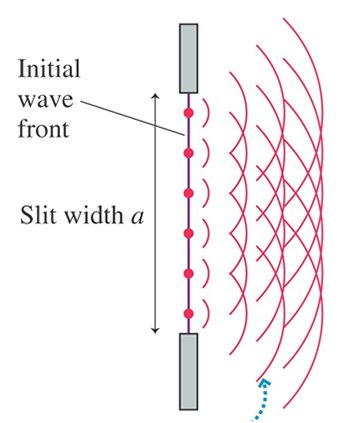
\includegraphics[scale=0.4]{Huygens.png}
	\caption[Huygens principle visualization]{Example of single slit diffraction described using Huygens principle. Image taken from \citep{Huygens}, where the principle is discussed further.}
	\label{fig: Huygens principle}
\end{figure}

Studying diffraction is crucial for understanding the nature of light. As diffraction is caused by constructive and destructive interference it has historically been used as a conclusive argument for the wave-behavior of light, as early as 1817 when looking at Argo spots (\citep{wiki:Arago}). Diffraction plays a huge part in all astronomy observations, as the effect limits the resolution of telescopes and the different instruments used to capture exposures. Understanding the limits of this angular resolution is important for construction of observatories and in the interpretation and analysis of the data from observations with disturbances from dust and other perturbations in the instruments.

\section{Data}
\label{sec:data}
\subsection{Single slit setup}
\label{subsec: Data/single slit setup}
For the single slit experiment we used a simple setup of a Helium-Neon laser with a wavelength of $\lambda_1 = 632.8$ nm mounted on a platform and powered by a $4.5$ V flat battery. Another platform was used to hold a $a_s=100 \, \mu$m opening slit in a fixed position in the light path from the laser, projecting a diffraction pattern on a wall a distance $L_s = 147.5 \pm 1.5$ cm from the slit. Schematic of the setup in \cref{fig: Setup slit}, where I've included the expected diffraction pattern.


We replaced the platform holding the slit with a new platform holding a Norwegian paperclip, functioning as an anti-slit. Using a caliper we measured the width the paperclip to $a_a = 0.89 \pm 0.02 $ mm (\cite{SuperCaliper}). The anti-slit was placed a distance $L_a = 200 \pm 2.0$ cm from the wall.

\subsection{Circular aperture setup}
\label{subsec: Data/circular setup}
Here we used a Helium-Neon laser with wavelength $\lambda_2 = 635$ nm powered by an external power supply. We used a circular doublet lens, with a focal length $f=100$ mm and diameter $d = 5.0 \pm 0.2$ cm, focusing the light and producing an Airy disc. A microscopic objective with a $M = 20x$ magnifying effect and a monochromatic camera with $p=6 \, \mu$m pixels takes the exposure. A schematic of the setup is included in \cref{fig: Setup circular}.

\begin{figure}
	\centering
	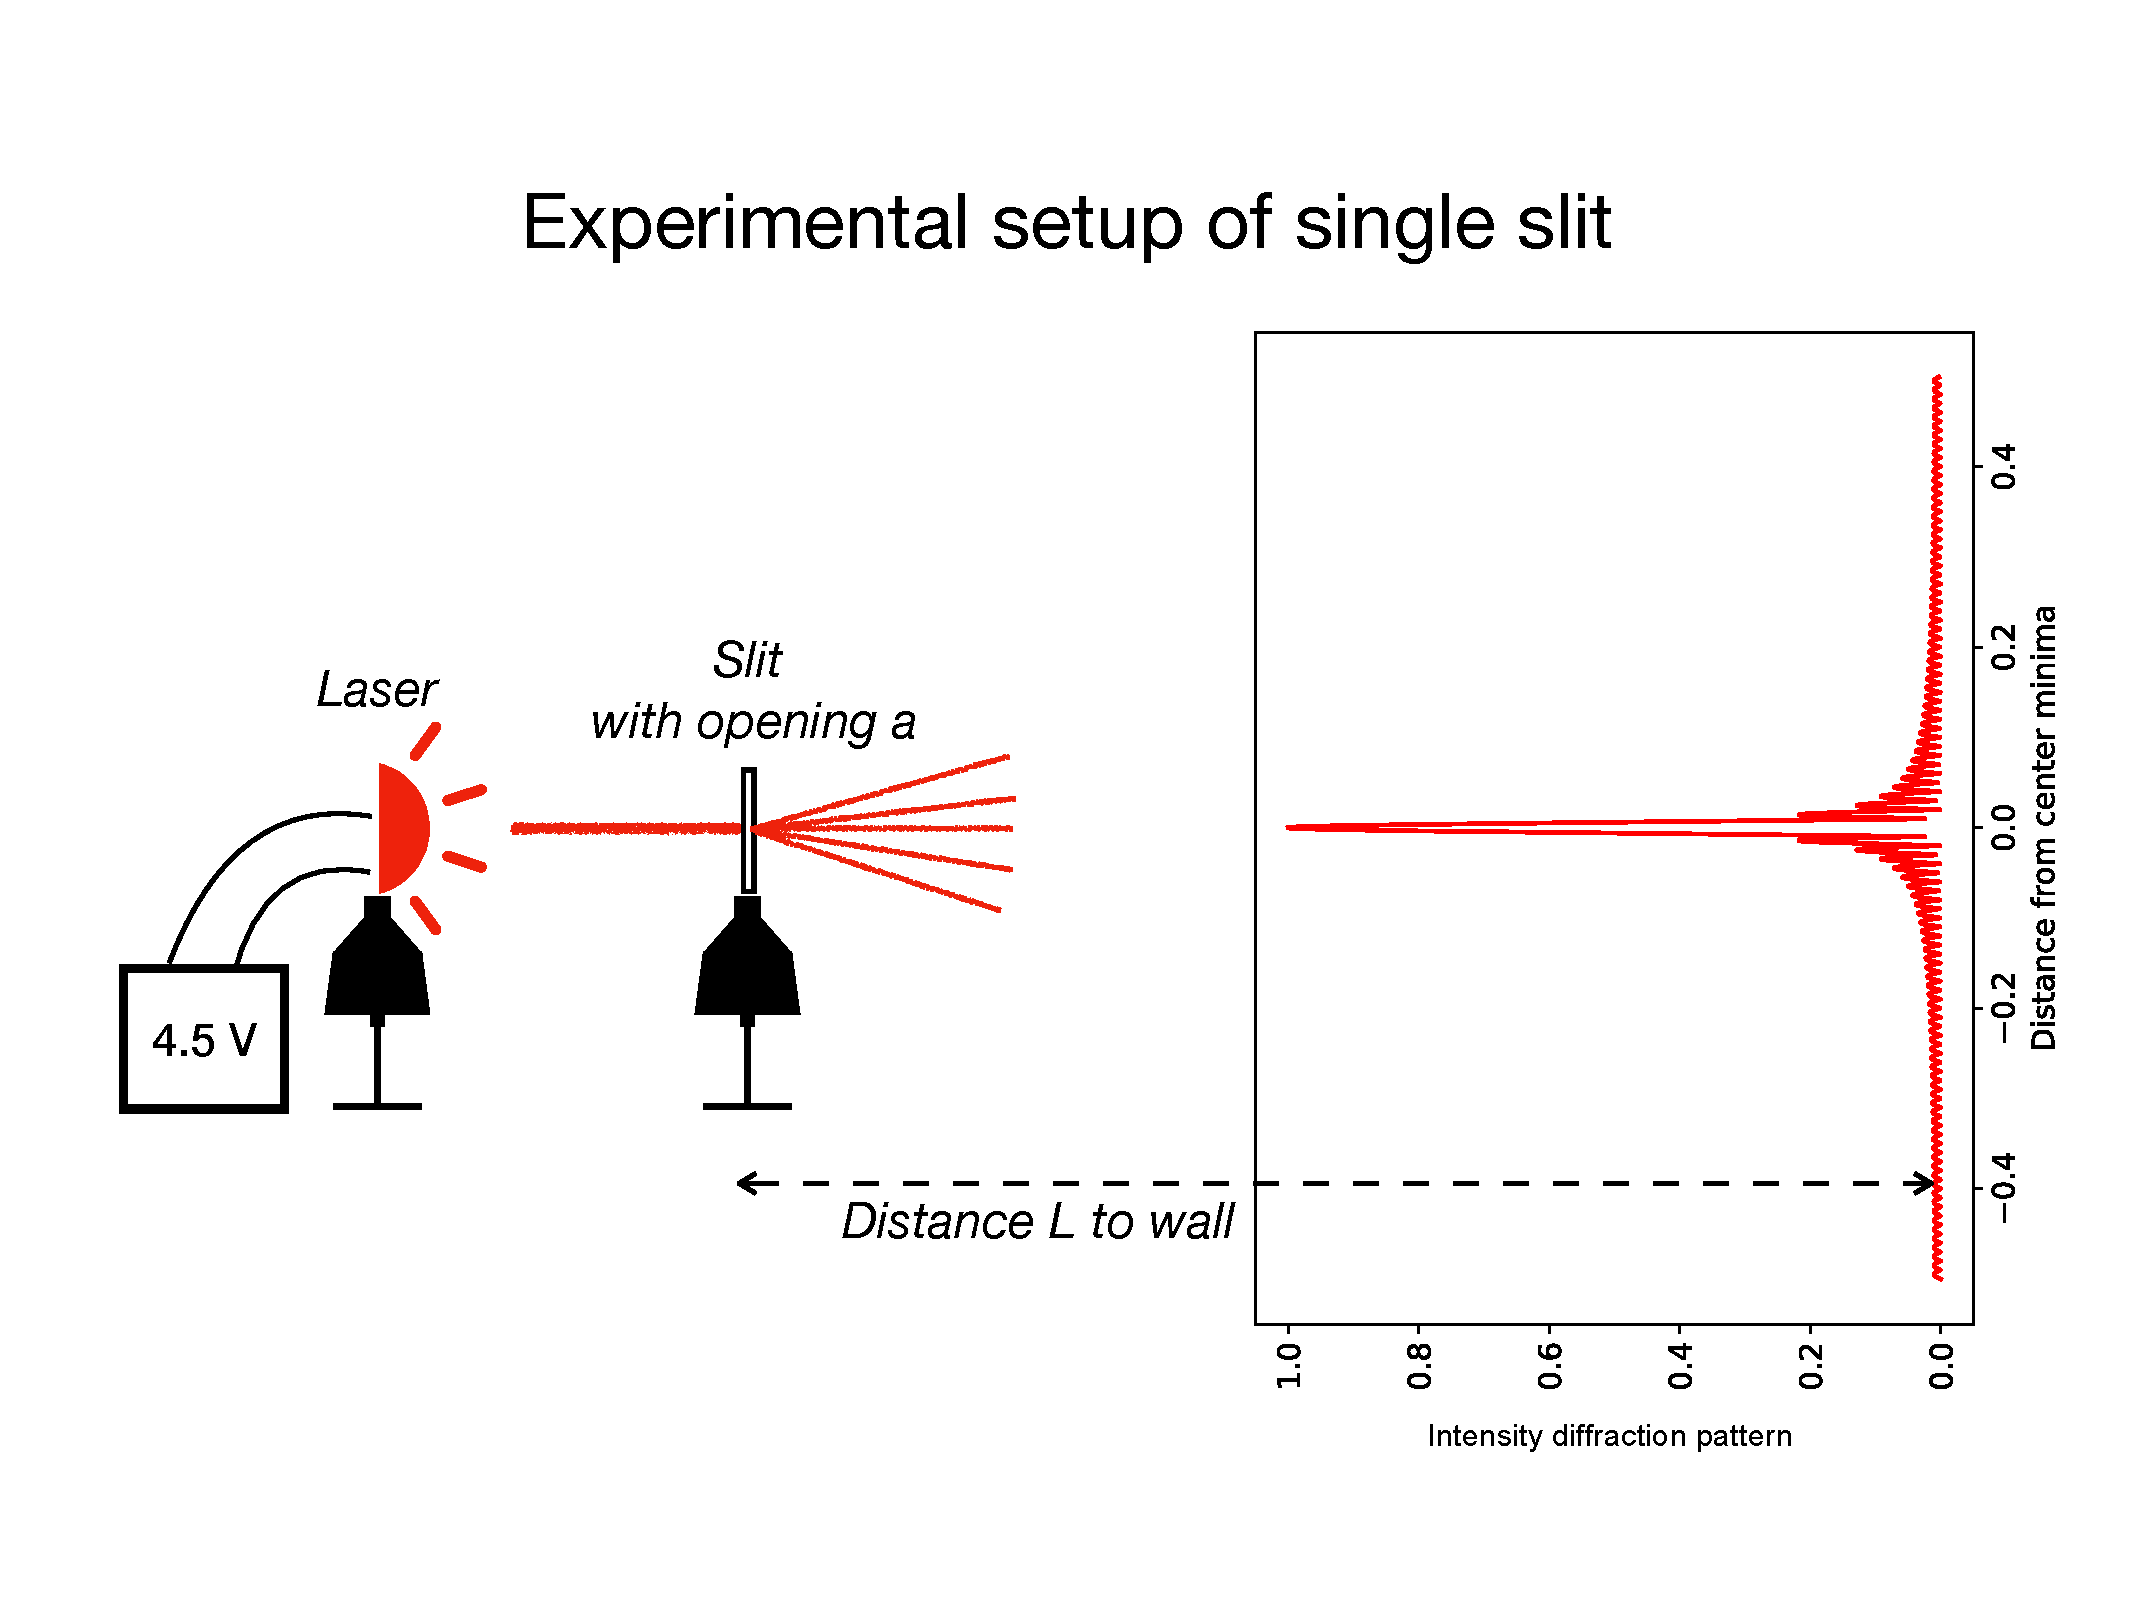
\includegraphics[width=\linewidth]{exp_setup.pdf}
	\caption[Experimental setup single slit]{Schematic of experimental setup for the single slit diffraction experiment. Two platforms holding the slit and the laser, with a $4.5$ V battery. The slit projects a diffraction pattern on the wall a distance $L$ from the slit. The expected intensity of the diffraction pattern produced by a general slit is shown on the right.}
	\label{fig: Setup slit}
\end{figure}

\begin{figure}
	\centering
	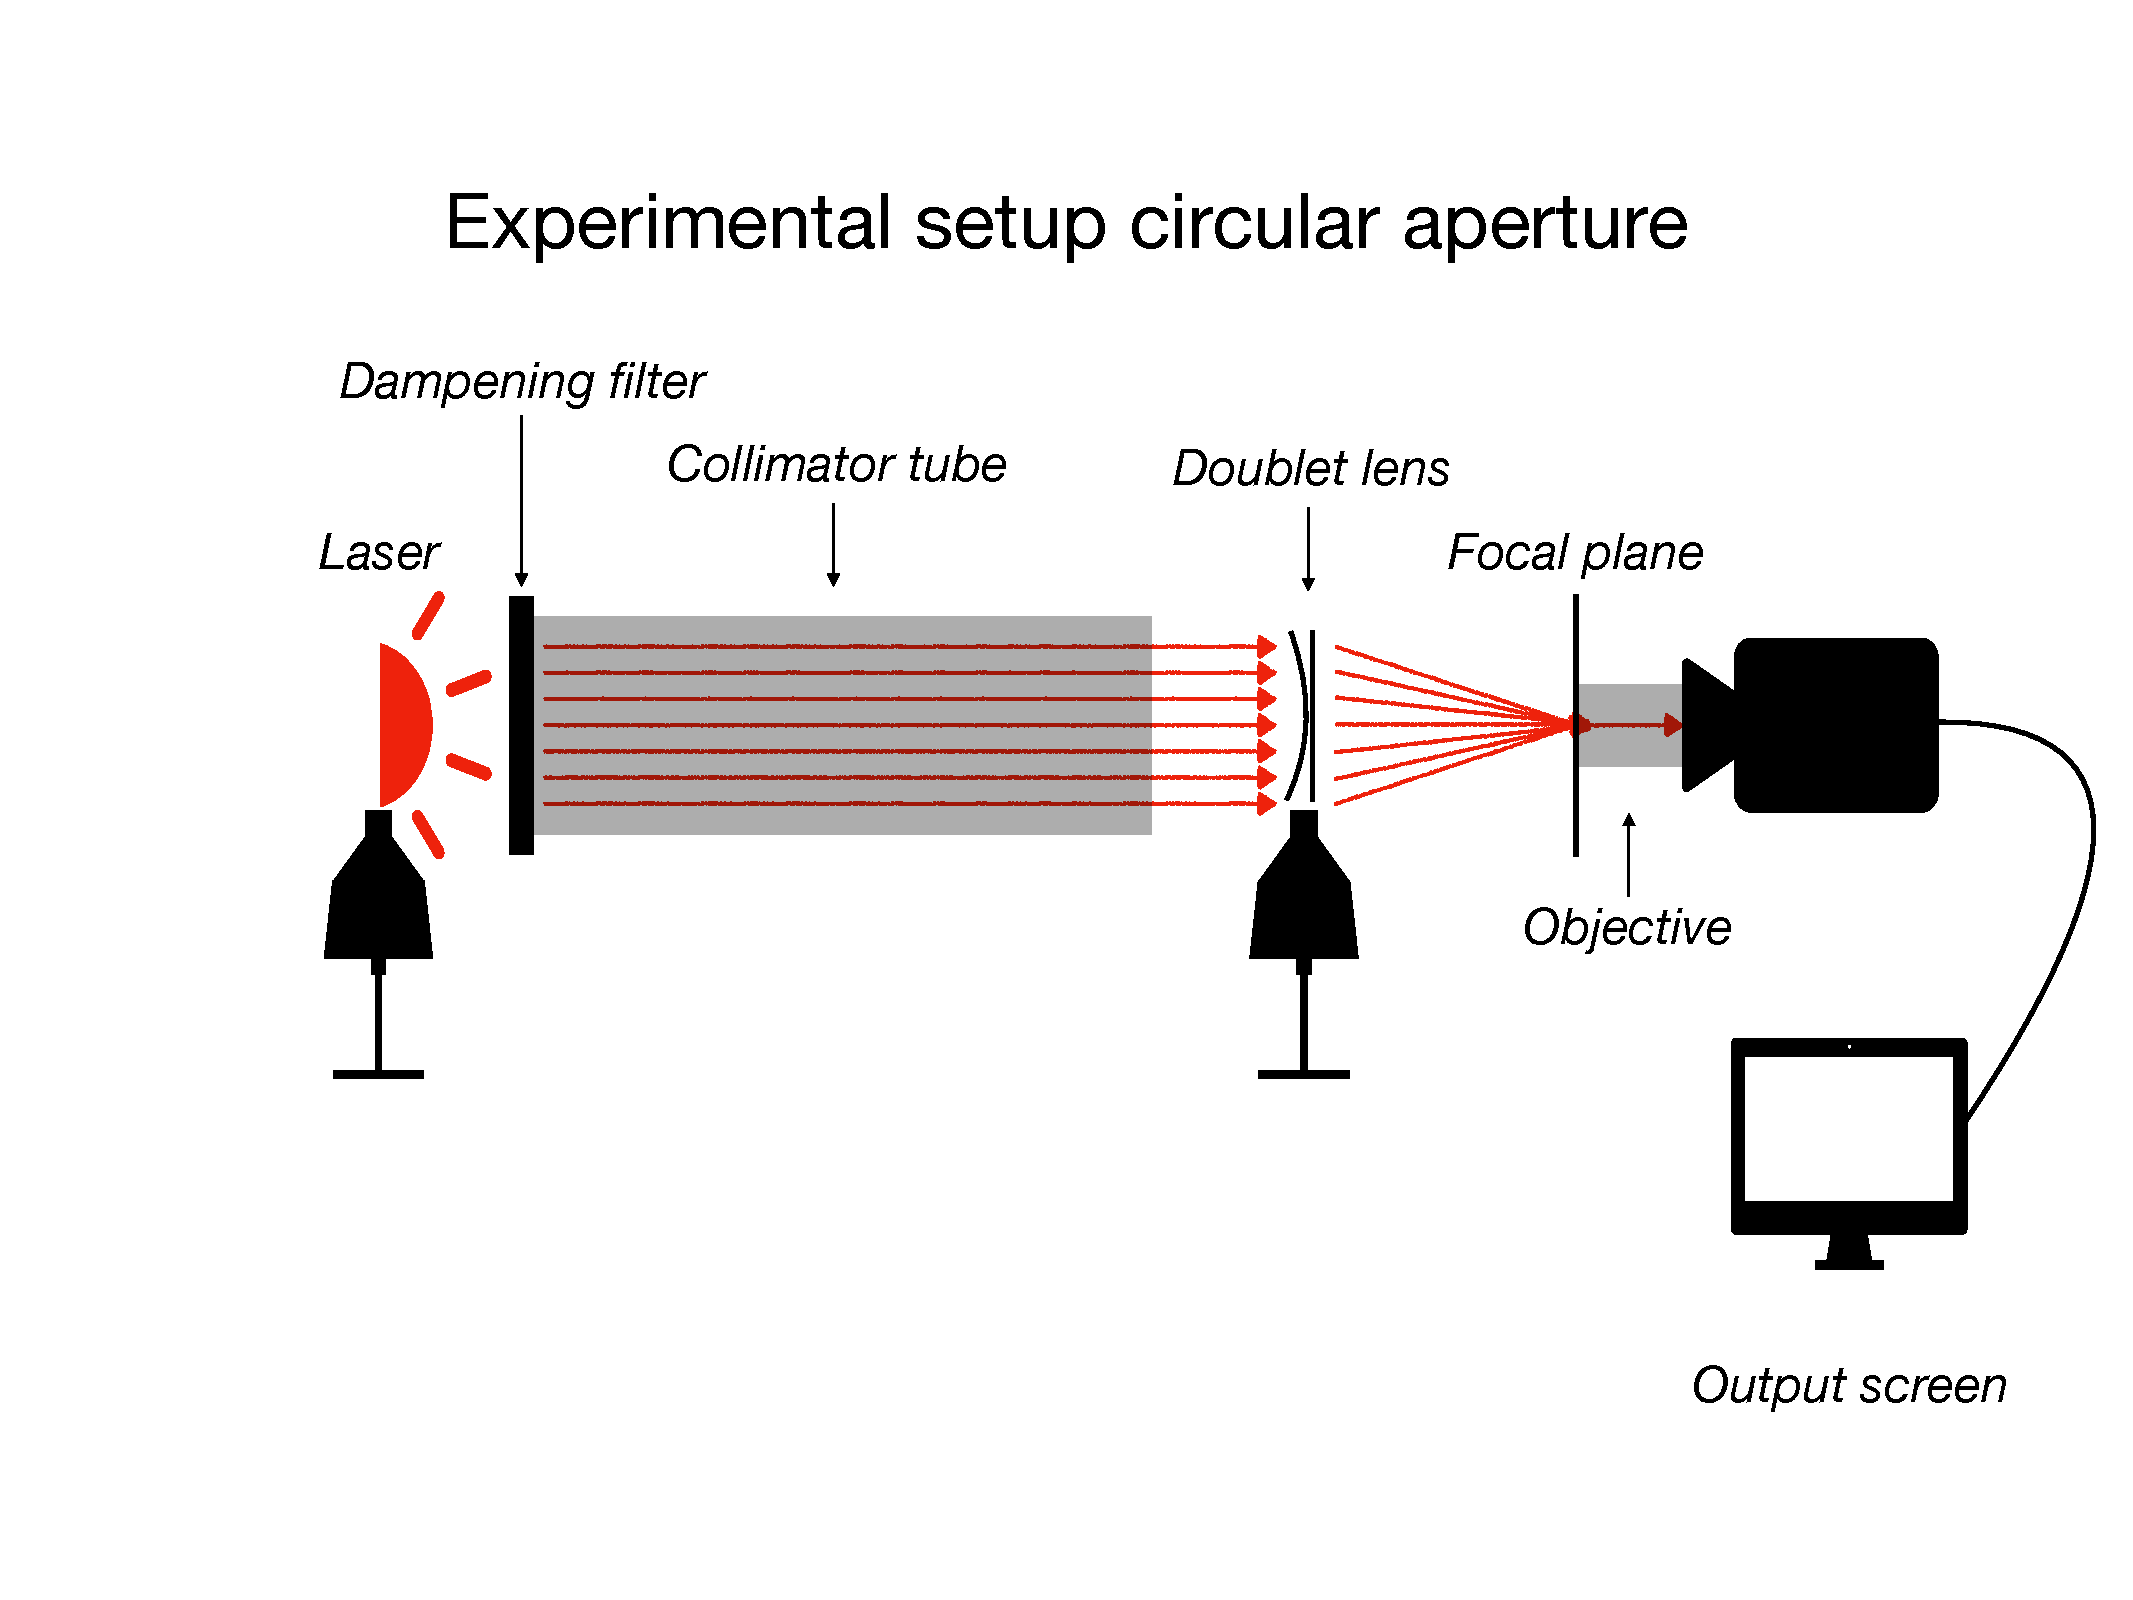
\includegraphics[width=\linewidth]{circ_setup.pdf}
	\caption[Experimental setup circular aperture]{Schematic of experimental setup for the circular aperture diffraction experiment. The laser intensity is reduced in the dampening filter so that the camera is able to differentiate the signal. The light is then made parallel in a collimator tube, and focused by the doublet lens producing an airy disc. The objective is placed in the focal plane of the lens to magnify the exposure for the camera. We can then observe the magnified airy disc on the computer screen.}
	\label{fig: Setup circular}
\end{figure}

\begin{figure}
	\centering
	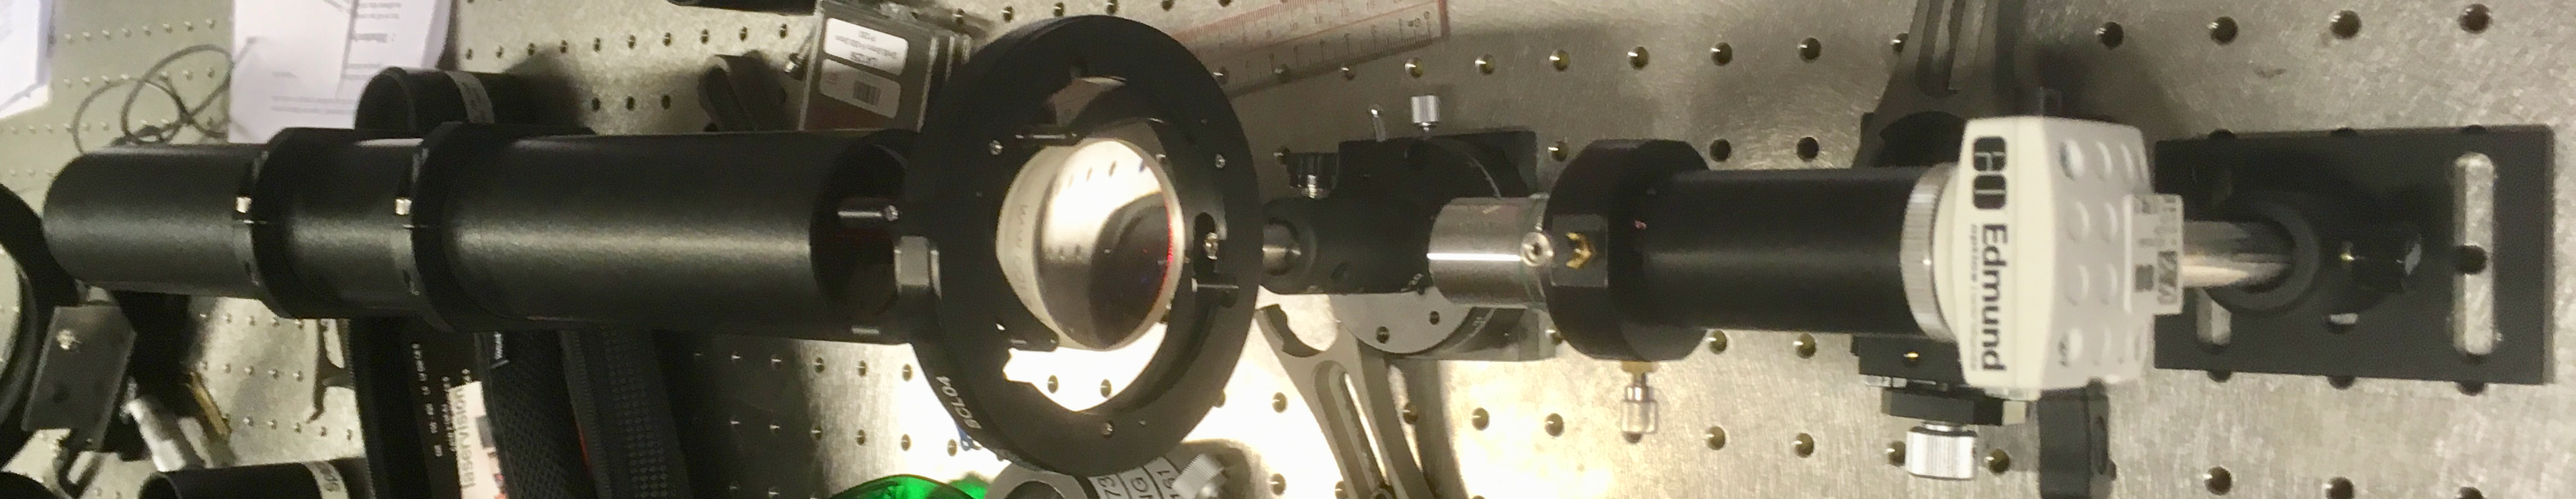
\includegraphics[scale=0.05]{circ_setup.png}
	\caption[Experimental setup circular aperture]{Photo of setup described in \cref{fig: Setup circular} for the circular aperture.}
	\label{fig: Setup circular photo}
\end{figure}

\section{Method}
\label{sec:method}
\subsection{Single slit experiment}
\label{subsec: Method Single slit}
With the laser and slit in place, we can connect the battery and observe the diffraction pattern on the wall. We projected the positions of the minimas on to a white paper. We then measure the length, $y_s = 11.5 \pm 0.35$ cm, from the center of the pattern to the furthest away minima we could clearly define, that is minima of order $m_s=12$. Together with the distance from the slit to the wall, $L_s$ which was measured using a normal tape measurer, and the slit width, $a_s$, we can experimentally find the wavelength of the Helium-Neon laser using the equation for single slit diffraction
\begin{equation}
a\sin(\theta) = m\lambda.
\label{eq: Single slit diffraction}
\end{equation}

Here we can find the angle $\theta$ from our measurements of $y_s$ and $L_s$ through $\tan(\theta) = \frac{y}{L}$, demonstrated in \cref{fig: Geometric single slit}. Also, if the angle $\theta$ is small enough we can use the small angle approximation, which is valid if 
\begin{equation}
\sin(\theta) \approx \tan(\theta) \approx \theta.
\label{eq: Small angle approximation}
\end{equation}
This approximation simplify a lot as we don't have to propagate the uncertainties through both the arc-tangent and sinus functions. If we can use the small angle approximation \cref{eq: Single slit diffraction} becomes
\begin{equation}
a\theta = m\lambda.
\label{eq: approx single slit diffraction}
\end{equation}

When we have measurements for the wavelength of the laser we replace the slit with an anti-slit in the form of a paperclip. We had to move the platform and the laser further from the wall, a distance $L_a$, to easier resolve the diffraction pattern produced. With the same procedure as for the single slit, we find the distance $y_a = 2.7 \pm 0.2$ cm from the center out to minima of order $m_a = 18$. Using \cref{eq: Single slit diffraction}, we experimentally calculate the width $a_a$ of the paperclip from the diffraction pattern produced on the wall.
\begin{figure}
	\centering
	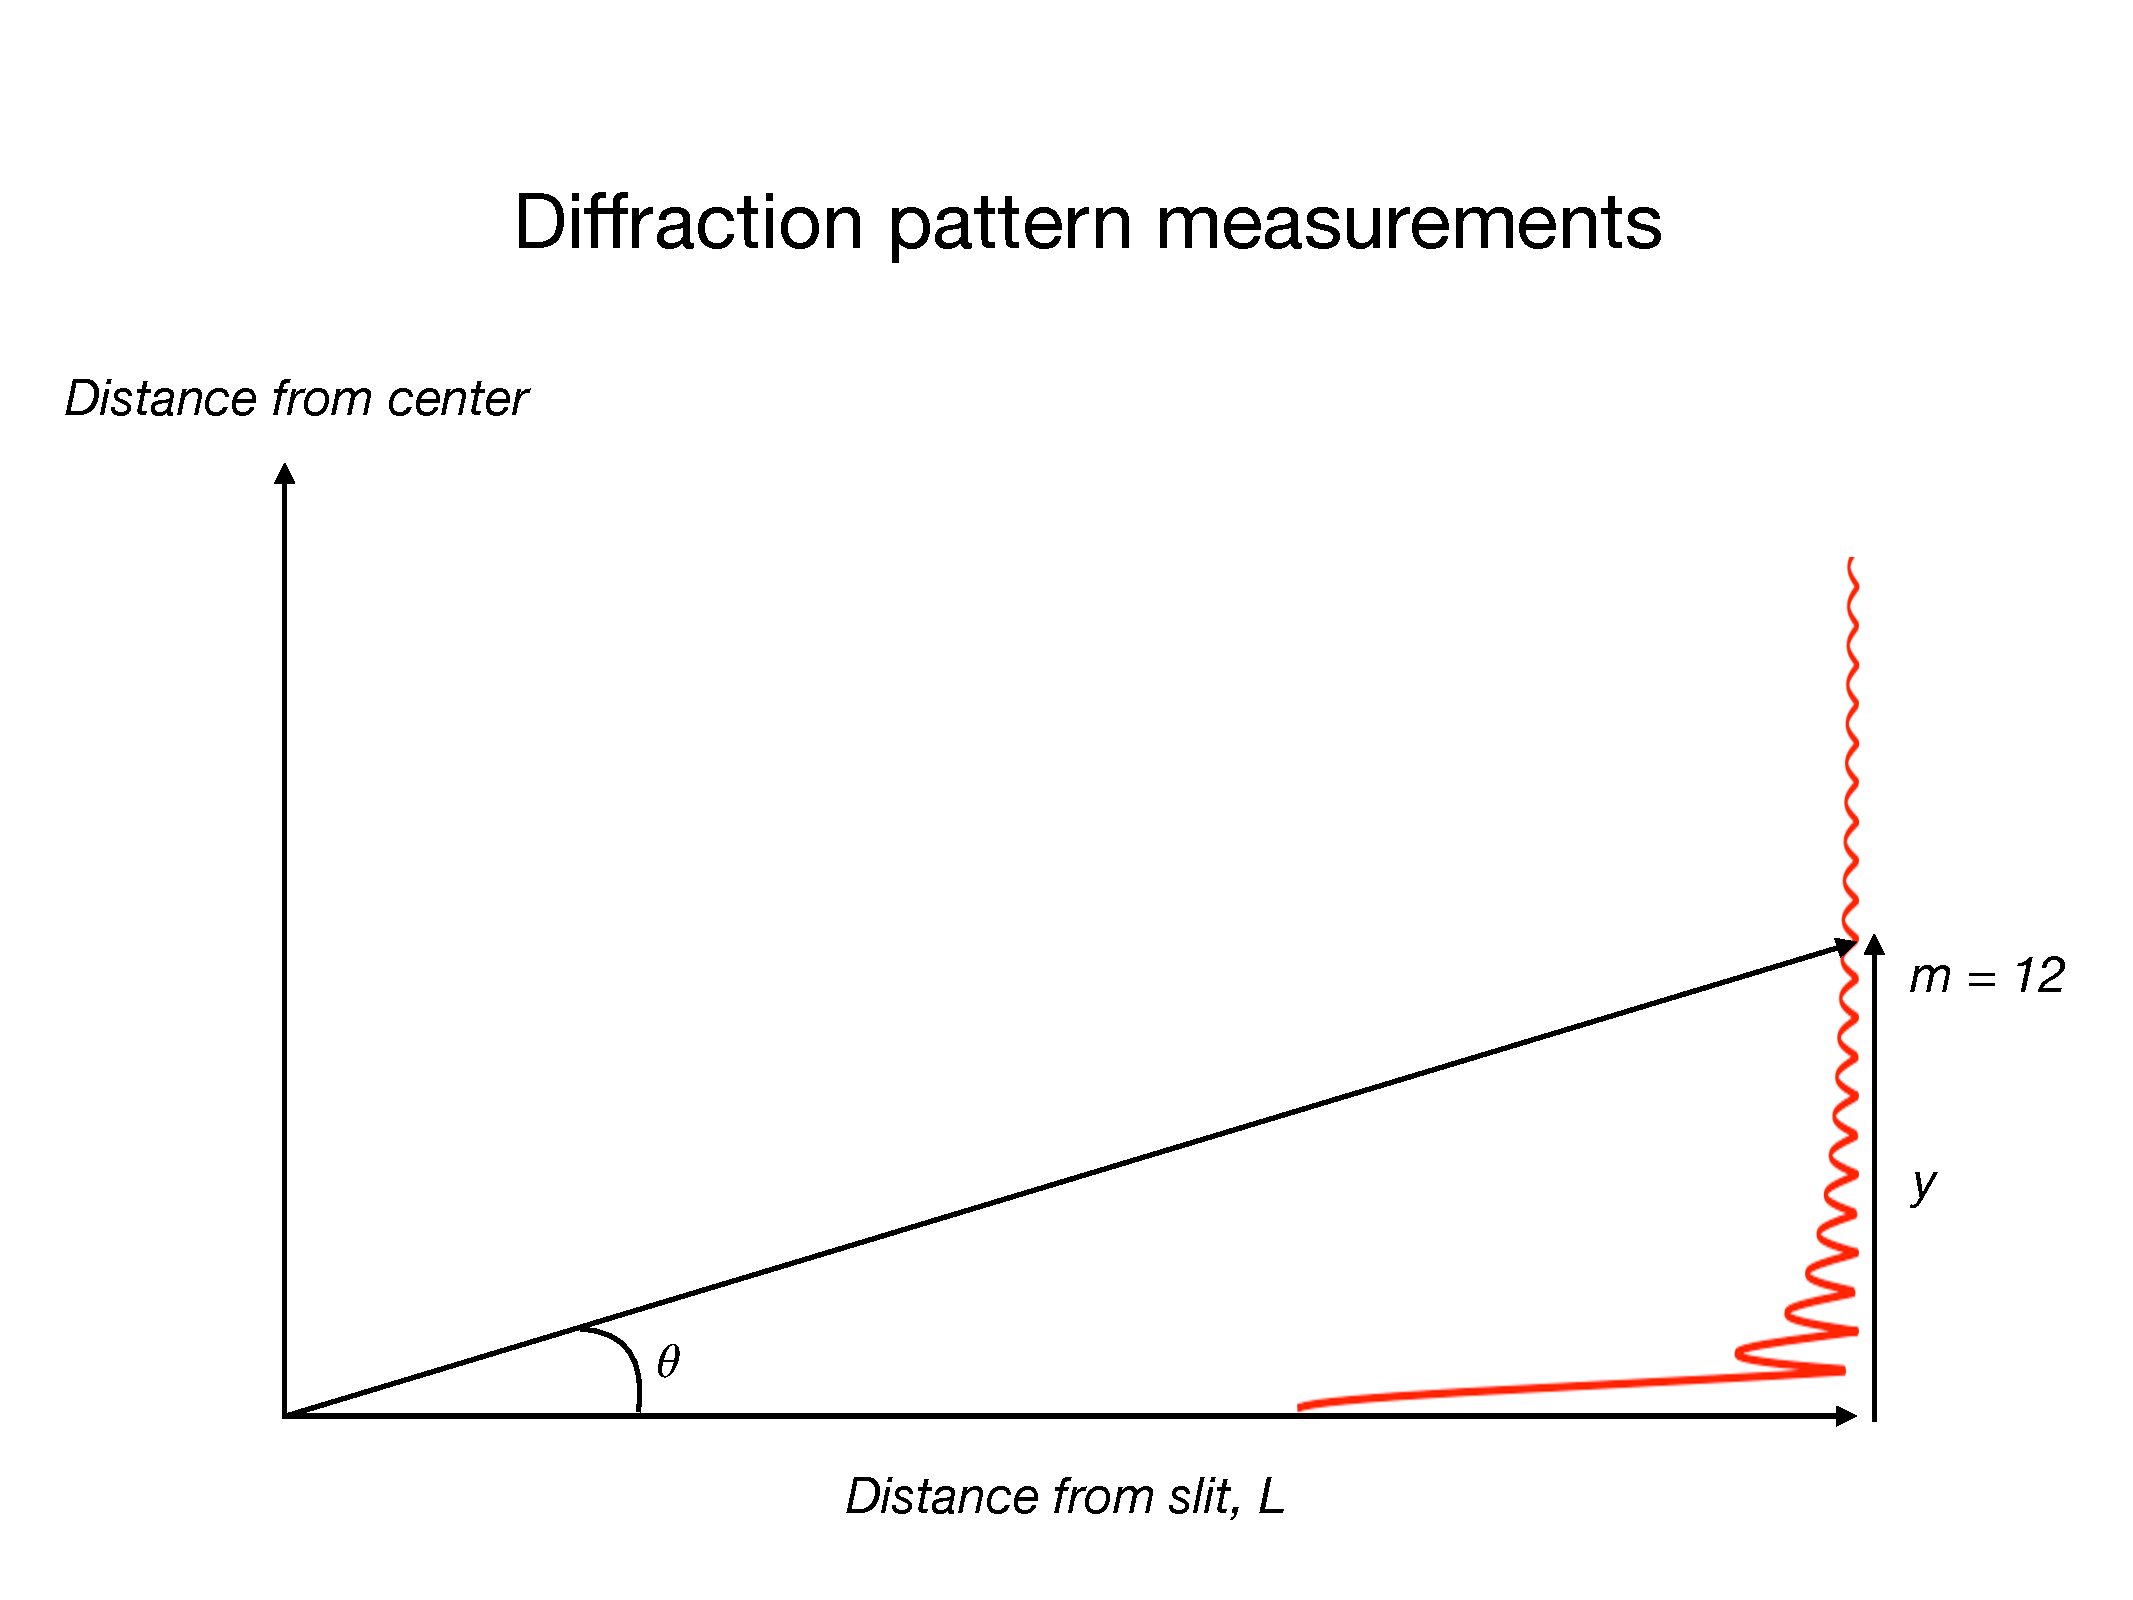
\includegraphics[width=\linewidth]{diff_measurements.pdf}
	\caption[Geometric measurements in diffraction pattern]{Demonstrating the general procedure for finding the angle from the center in a diffraction pattern. Here displayed for the single slit case. The angle $\theta$ is found with $L$ from the slit to the wall $L$ and $y$ from the center of the pattern to minima number $m$. The same technique can be applied for different patterns.}
	\label{fig: Geometric single slit}
\end{figure}

\subsection{Circular experiment}
\label{subsec: Method/Circular experiment}
The laser is made parallel through a collimator tube with a dampening filter such that the camera is able to distinguish the different intensities in the exposure. The parallel light is focused with the circular doublet lens, and the objective placed in the focal plane with the camera attached. 

The lowest image resolution of a lens of diameter $d$ when observing light of wavelength $\lambda$ is determined by Rayleigh's criterion
\begin{equation}
\sin(\theta_1) \approx \theta_{1} = K_1 \frac{\lambda}{d}
\label{eq: Rayleighs critterion}
\end{equation}
Here we apply the small angle approximation right away, as we know we are far in the Fraunhofer regime and the angle is tiny. This equation can be expanded to look at different ordered minimas
\begin{equation}
\theta_{i} = K_i \frac{\lambda}{d} \qfor i = 1,\, 2,\, 3,\, \ldots \text{ .}
\label{eq: Airy disc minimas}
\end{equation}

In our case we have been given the value of the first empirical constant $K_1 = 1.22$ which we can use to determine the wavelength of our Helium-Neon laser from \cref{eq: Rayleighs critterion}. For measuring the distance $y_{c,i}$ from the center of the Airy disc to the second and third minima we count the number of pixels $n_i$ in our exposure as shown in \cref{fig: Airy pixel}. In the same way as in \cref{subsec: Method Single slit}, we find the angles $\theta_{1}$, $\theta_2$ and $\theta_3$ using the small angle approximation. With the angles for the first minima we find the wavelength of the laser, and with the second and third minima we find the values of the empirical constants $K_2$ and $K_3$ from \cref{eq: Airy disc minimas}.

We also captured an exposure of the dust in our optical system before we removed the dampening filter, lens, objective and camera to place a circular Norwegian $10$ NOK coin without central hole in the light beam. The coin acts as a circular shape and produces a diffraction pattern where we should be able to observe an Argo spot as described in \citep{wiki:Arago}. 

\section{Results}
\label{sec:results}
\subsection{Slit diffraction}
\label{subsec: Results/Slit}
\paragraph{Small angle approximation}
To handle the uncertainties we check if the small angle approximation is valid using criteria \cref{eq: Small angle approximation}. Results presented in \cref{tab:Small angel approximation}. To our degree of precision the small angle approximation is valid for the slit, and is even more accurate for the anti-slit.
\paragraph{Laser wavelength} Solving \cref{eq: approx single slit diffraction} for $\lambda$ gives an experimentaly found wavelength of the Helium-Neon laser
\begin{equation*}
\lambda_s = 648 \pm 20.8 \text{ nm}.
\end{equation*}

\paragraph{Anti-slit width} Solving \cref{eq: approx single slit diffraction} for $a$ gives an experimentaly found width of the paperclip
\begin{equation*}
a_a = 0.86 \pm 0.07 \text{ mm}.
\end{equation*}

\subsection{Airy disc}
\label{subsec: Result Airy disc}
Exposure of the Airy disc is shown in \cref{fig: Airy zoom}, while the image used for counting the number of pixels to the different minimas in \cref{fig: Airy pixel}. The exposure of the dust in the optical system displayed in \cref{fig: Airy dust}. Photo of the Arago spot we produced in \cref{fig: Arago}. 
\paragraph{Wavelength of laser} Solving \cref{eq: Rayleighs critterion} for $\lambda$ gives an experimentally found wavelength
\begin{equation}
\lambda = 614.75 \pm 122.95 \text{ nm}.
\label{eq: Results lambda airy}
\end{equation}
\paragraph{Empirical constants} Solving \cref{eq: Airy disc minimas} for $K_2$ and $K_2$ using measurements presented in \cref{tab:Airy disc} and the experimentally found wavelength $\lambda$ gives the empirical constants
\begin{align}
K_2 &= 1.96 \pm 0.46
\\
K_3 &= 2.68 \pm 0.59
\end{align}

\begin{deluxetable}{lccc}
\centering
%\tablewidth{0pt}
\tablecaption{\label{tab:Small angel approximation}}
\tablecomments{Controlling small angel approximation. As the criteria in \cref{eq: Small angle approximation} is fulfilled the approximation holds.}
\tablecolumns{4}
\tablehead{Experiment & $\tan(\theta) = \frac{y}{L}$ & $\theta=\arctan(\frac{y}{L})$ & $\sin(\theta)$}
\startdata
 Slit: & $\frac{y_s}{L_s} = 0.0780$ & $\theta_s = 0.0778$ & $0.0777$ \\
 \\
Anti-slit: & $\frac{y_a}{L_a} = 0.0135$ & $\theta_a = 0.0135$ & $0.0135$
\enddata
\end{deluxetable}

\begin{deluxetable}{lccc}
%\tablewidth{0pt}
\tablecaption{\label{tab:Airy disc}}
\tablecomments{Measurements and values from circular aperture used to determine the wavelength and empirical constants from our Airy disc.}
\tablecolumns{4}
\tablehead{$i$  & $n_i$ & $y_{c,i}$ & $\theta_i$}
\startdata
$1$ & $5 \pm 1$ & $1.5 \pm 0.3 \, \mu$m & $\qty(1.5\pm 0.3) \cdot 10^{-5}$ \\
\\
$2$ & $8 \pm 1$ & $2.4 \pm 0.3 \, \mu$m & $\qty(2.4\pm 0.3) \cdot 10^{-5}$ \\
\\
$3$ & $11 \pm 1$ & $3.3 \pm 0.3 \, \mu$m & $\qty(3.3\pm 0.3) \cdot 10^{-5}$
\enddata
\end{deluxetable}

\begin{figure}
\centering
\includegraphics[width=0.82\linewidth]{airydisczoon.pdf}
\caption[Airy disc]{Captured exposure of Airy disc produced in the circular aperture experiment from \cref{subsec: Method/Circular experiment}.}
\label{fig: Airy zoom}
\end{figure}

\begin{figure}
\centering
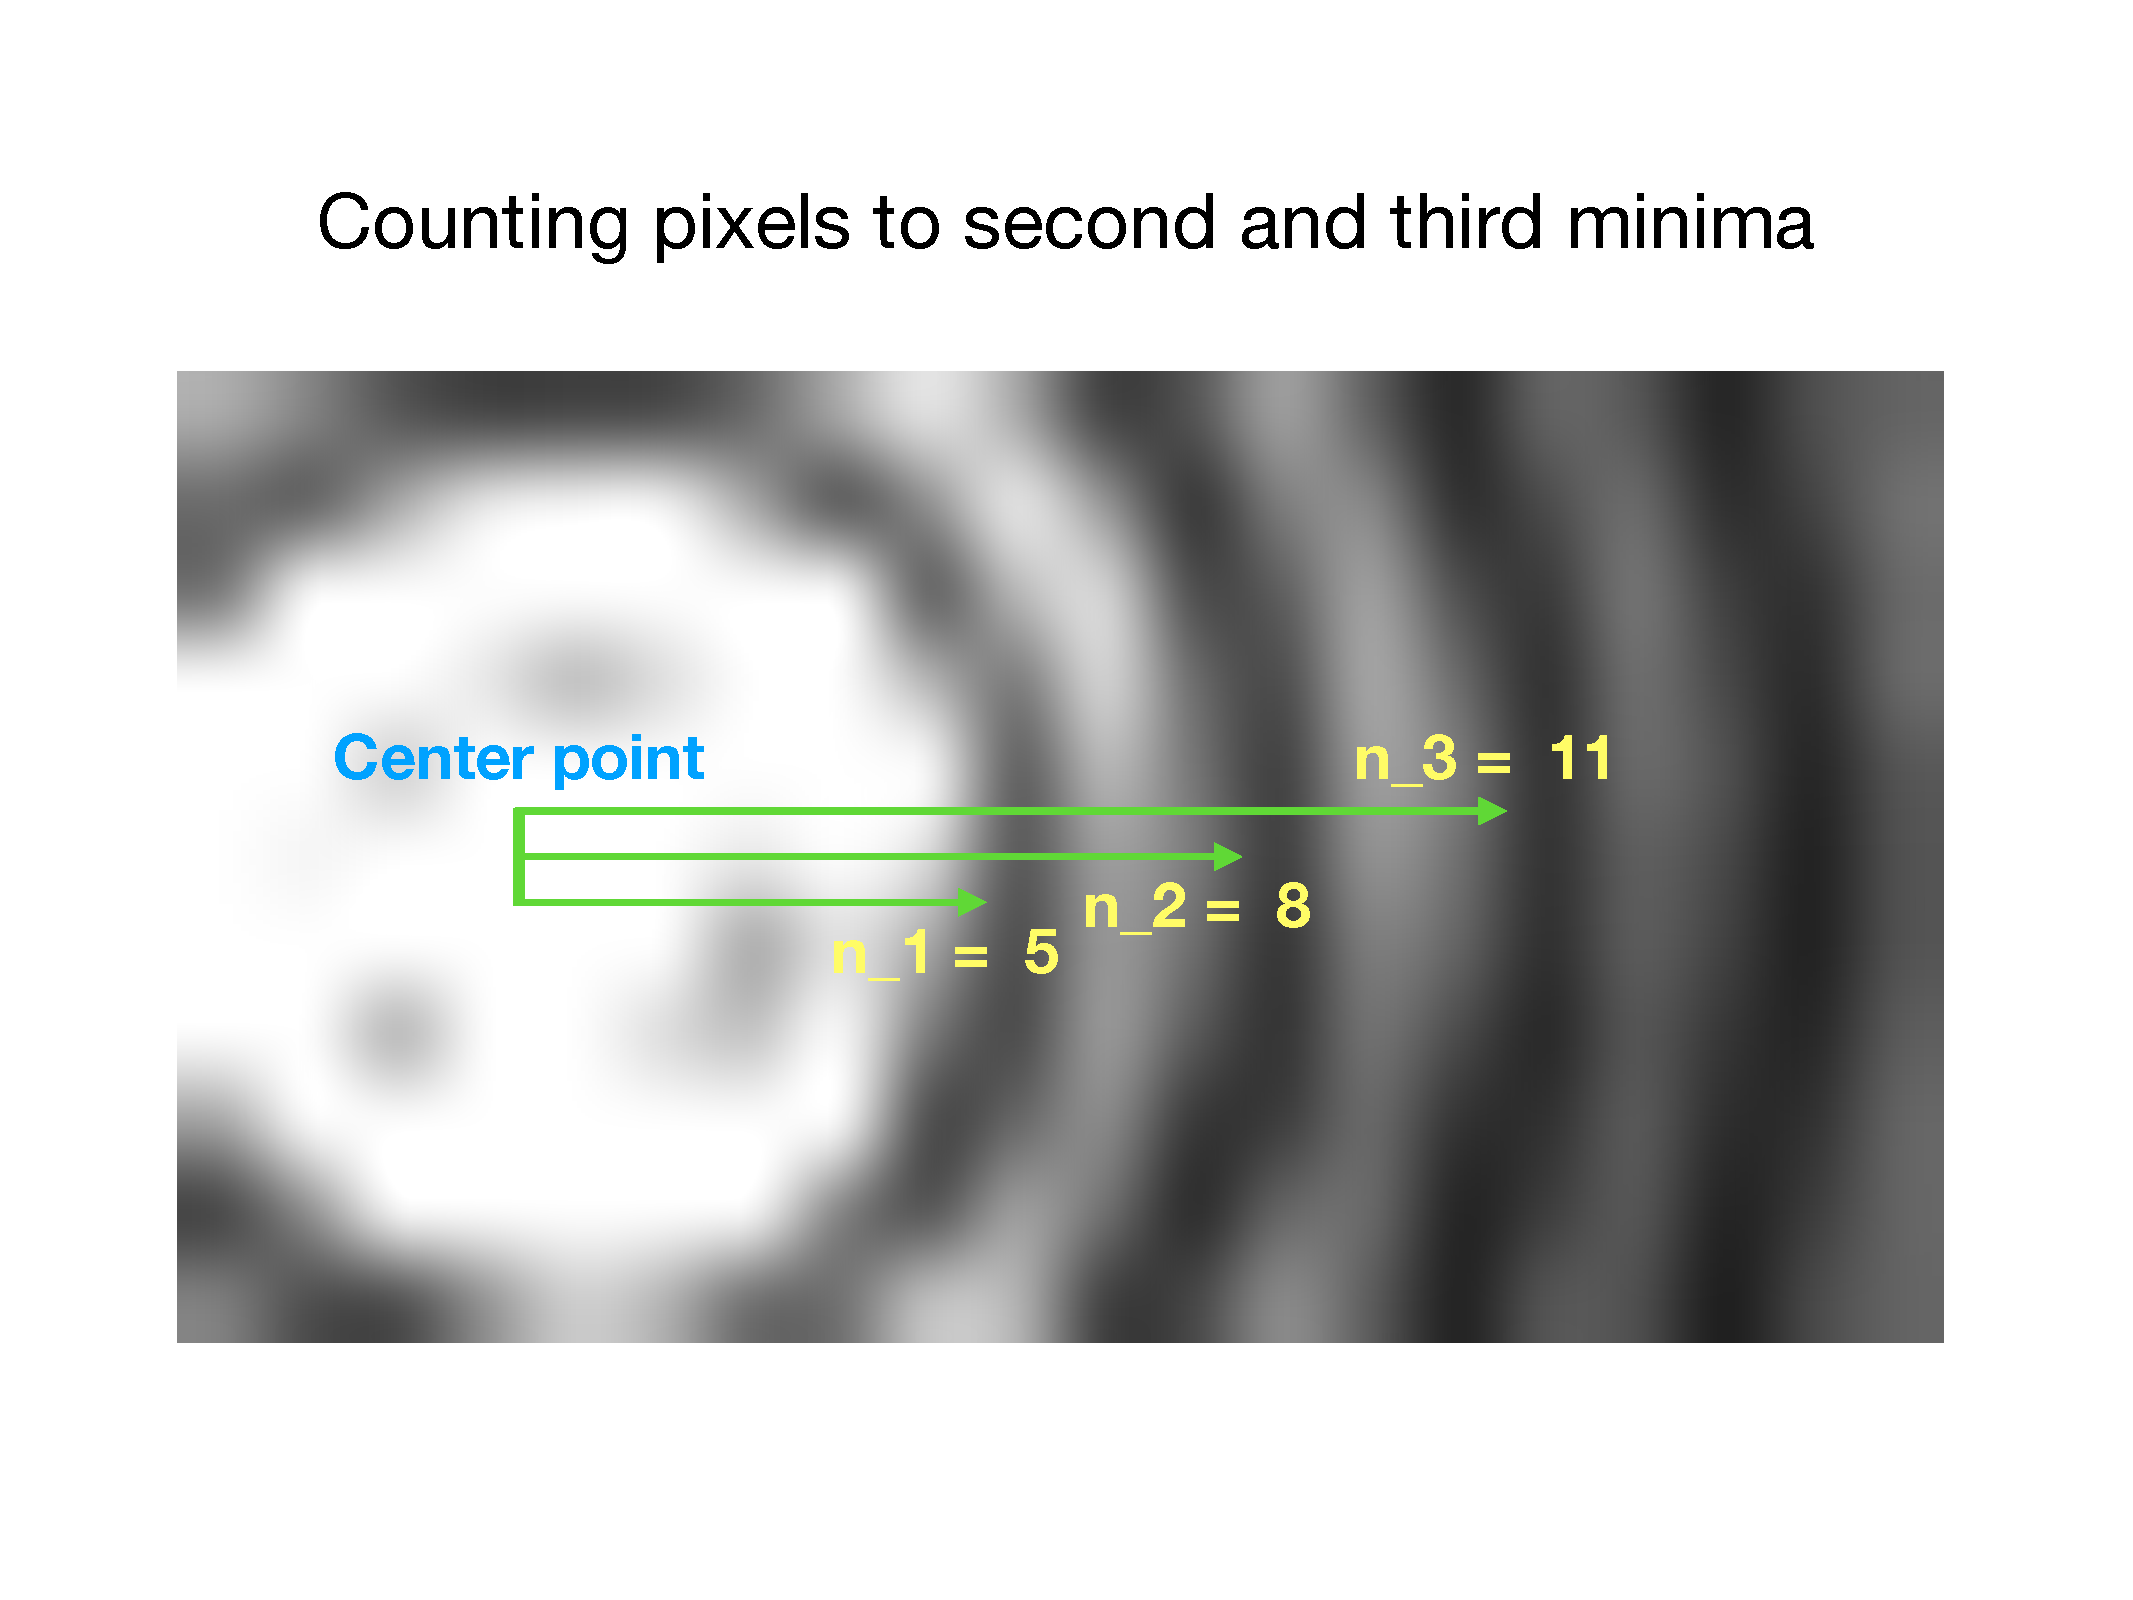
\includegraphics[width=\linewidth]{airypixelcount.pdf}
\caption[Airy pixel count]{Zoom in on airy disc in the exposure from \cref{fig: Airy zoom}. Here we count the number of pixels from the center to the first,second and third minima. We find $n_1 = 5$,$n_2 = 8$ and $n_3 = 11$.}
\label{fig: Airy pixel}
\end{figure}

\begin{figure}
\centering
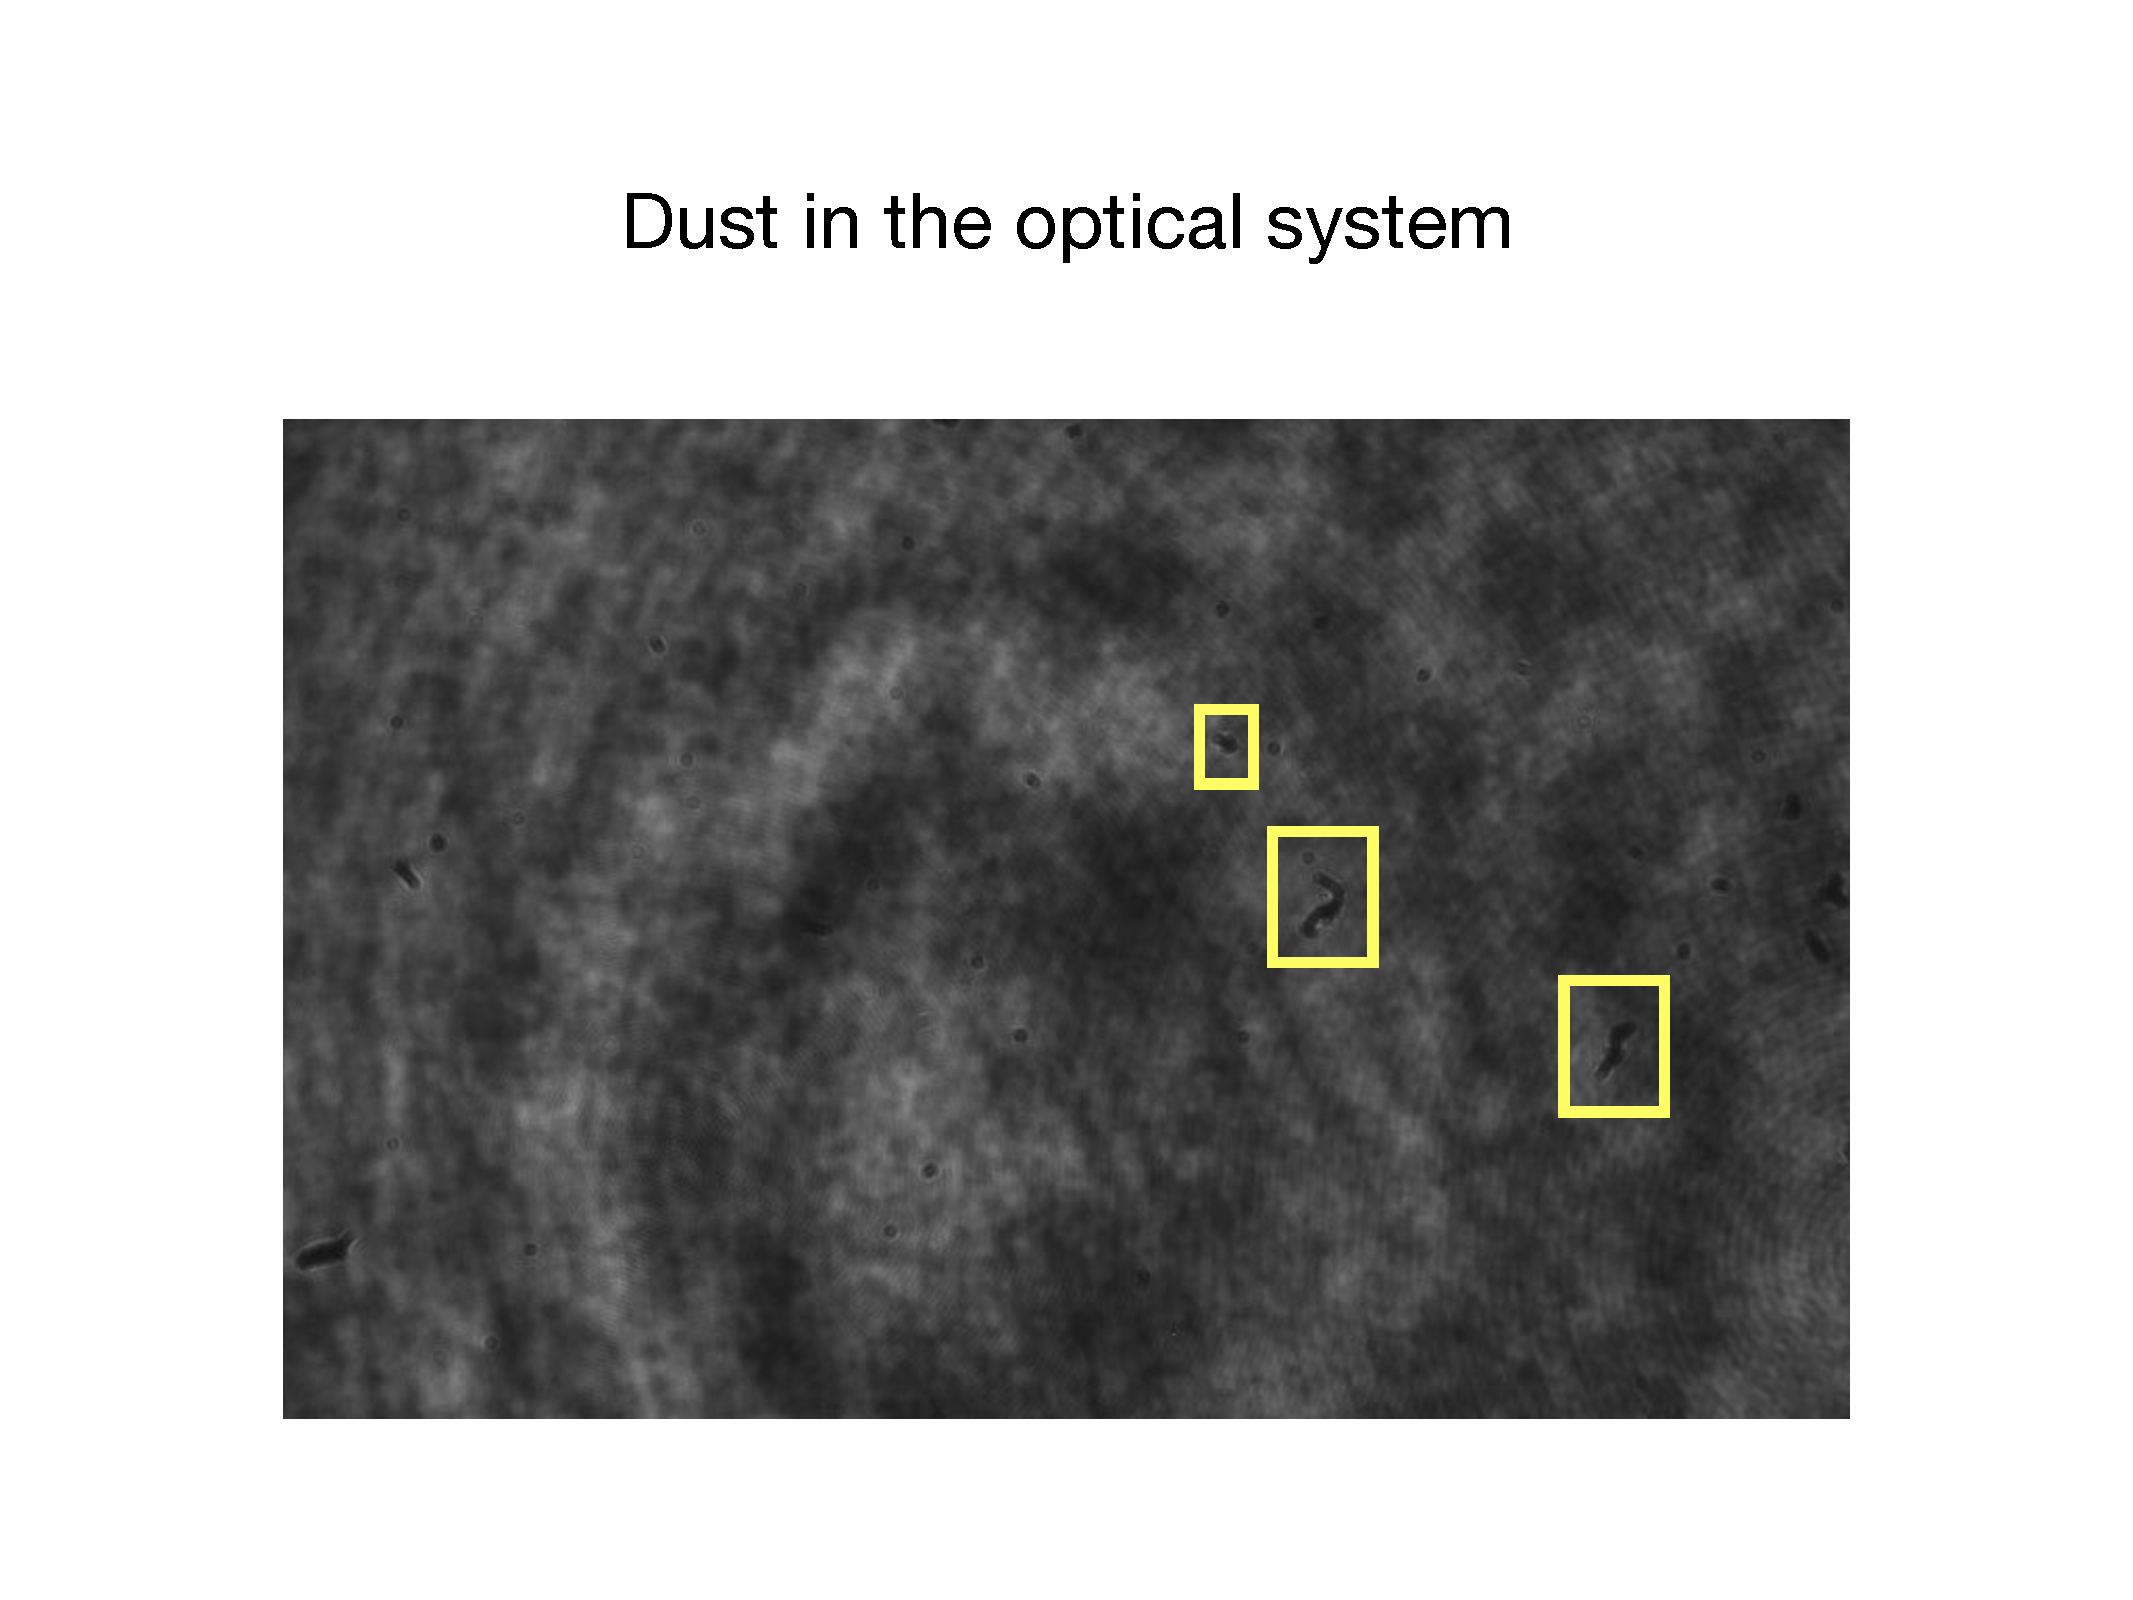
\includegraphics[width=\linewidth]{dust.pdf}
\caption[Optical disturbance from dust]{Captured exposure displaying the dust in the optical system used in \cref{subsec: Method/Circular experiment}. Some of the dust particles are highlighted with yellow squares.}
\label{fig: Airy dust}
\end{figure}

\begin{figure}
\centering
\includegraphics[scale = 0.05]{Arago.png}
\caption[Arago spot]{Photo taken of the Arago spot produced using the coin mentioned in \ref{subsec: Method/Circular experiment}. Notice the tiny red spot in the center.}
\label{fig: Arago}
\end{figure}

\section{Conclusions}
\label{sec:conclusions}
\subsection{Understanding diffraction}
How diffraction affects light is crucial for observational astronomy. In this project we have studied some of the most general concepts of diffraction though different experiments to strengthen our general understanding of the concept and effects.
In general, the shape of the diffraction pattern from a specific aperture can be obtained from the Fourier transformation of the shape of the aperture. An example in the simple case of the single slit is included in \cref{fig: FFT single}.
\begin{figure}
\centering
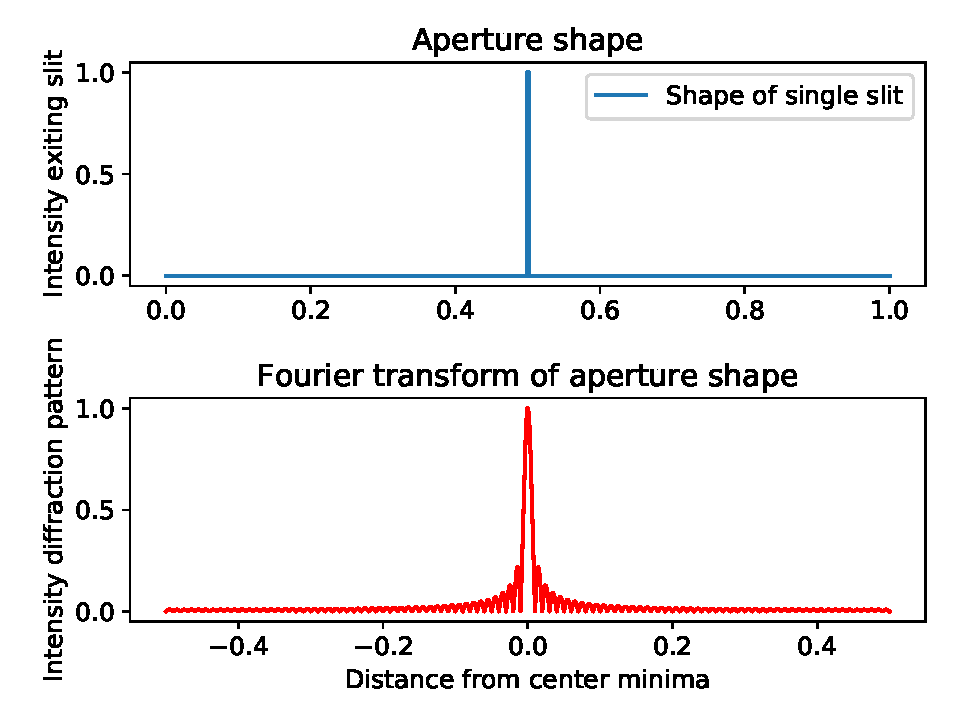
\includegraphics[width=\linewidth]{FFT_single_slit0.pdf}
\caption{Example of the Fourier transform of the shape of an aperture, here displayed in the case of the single slit, obtained numerically using the "Fast Fourier transform" algorithm from the numpy library. In the upper image the single slit shape is plotted as the normalized intensity of the light passing through. The lower image shows the diffraction pattern produced as the Fourier transformation of the signal of intensity from the slit. The distance from center minima is not to scale.}
\label{fig: FFT single}
\end{figure}

\subsection{Single slit and anti-slit diffraction}
From our single slit diffraction experiment we used \cref{eq: Single slit diffraction} to determine the wavelength of our Helium-Neon laser and found $\lambda_s = 648 \pm 20.8$ nm. This is as expected, within uncertainties, as the known wavelength for this red laser was $\lambda = 632.8$ nm.
We found the width of the anti-slit, $a_a = 0.86 \pm 0.07$ mm, which is well within uncertainties as expected from the measurements with the caliper. We also observed the expected diffraction pattern, the complimentary pattern of that of the single slit, we knew from Babinet's principle \citep{swaves}.
For future reproductions of these experiments we could have gotten better result with less uncertainty if we used better measurement techniques. For example we could have measured the distances from the aperture to the wall with a laser measuring tool. Further improvements could been made if when measuring the distance from center to minima $m$, we instead used the distance from minima $m$ to the same order minima on opposite side of the center and divided the distance by two.

\subsection{Circular diffraction}
From our circular diffraction experiment we used \cref{eq: Airy disc minimas} to find the empirical constants used to describe the second and third order minima in an Airy disc. We found $K_2 = 1.96 \pm 0.46$ and $K_3 = 2.68 \pm 0.59$. The Airy disc limits the lowest resolution of telescopes observing point like light sources such as stars. If two such sources lay close enough such that their Airy discs overlap it will not be possible to distinguish them. The values found here for $K$ are only valid for the monochromatic light used here with the specific wavelength $\lambda = 614.75 \pm 122.95$ nm. For a future experiment it would be interesting to do the same procedure with multiple lasers of different wavelengths to produce a range of $K$-values for the hole visible spectrum.
The uncertainty in our results for the empirical constants is quite large, as it is propagated  from the huge uncertainty in our measurements of the wavelength $\lambda$. The main contributor to this uncertainty is the counting of pixels in \cref{fig: Airy pixel}, which could been improved using a camera with a higher number of pixels. Indeed we could have included a slightly higher uncertainty if we also used uncertainty in the distance from the lens to the objective. In the calculations of the angles to the three different minimas we used the exact value for the focal length of the lens, but compared to the uncertainty in the number of pixels this is negligible.

\subsubsection{Arago spot}
Interrupting the parallel light beam with a circular Norwegian coin produced a circular shadow with a tiny illuminated spot in the middle, the Arago spot, just as Fresnel's wave theory described in \citep{wiki:Arago} predicts. We did not conclude any interesting results of this part of the experiment, but recreated the historical effects studied by many physicist ever since the discovery of the wave nature of light.

\subsubsection{Dust in optical systems}
As displayed in \cref{fig: Airy dust} every disturbance in the trajectory of the light captured in an exposure may effect the results. From the tiny dust particles in our systems we can see small diffraction patterns developing around the particles. As these particles are opaque they produce the inverse of the pattern produced by an open aperture of the same shape, as predicted by Babinet's principle \citep{swaves}.

\subsubsection{Unfinished experiments}
With limited available time in the lab, we did not have time to study one last effect. By placing a circular aperture reducer in front of the lens we could have studied the Airy pattern from different sized apertures. Due to the smaller diameter $d$, equation \cref{eq: Rayleighs critterion} predicts that $\theta_{1}$ would increase, thus giving a poorer angular resolution.

\begin{acknowledgements}
Thanks to my colleagues and co-workers in the execution of the experiments: Joakim Flatby, Nils-Ole Stutze, Vadim Vladimirov, Jon Dahl and Bendik S. Dalen.\\
Thanks to our guide and supervisor in the lab: Souvik Bose.
\end{acknowledgements}

\bibliographystyle{plainnat}
\bibliography{ref}
\clearpage
\begin{appendices}
\section{Additional calculations including uncertainties}
\label{asec: Calculations}
\paragraph{Single slit laser wavelength in \cref{subsec: Results/Slit}} Using \cref{eq: approx single slit diffraction} and solving for $\lambda$ with uncertainties propagating from $\theta_s$
\begin{align*}
\qq*{finding $\lambda_S$:} & \lambda_s = \frac{a}{m}\theta = \frac{100 \cdot 10^{-6}}{12}\cdot 0.0778 \text{ m}= 648.33 \text{ nm}
\\
\qq*{uncertainty:} & \frac{\delta \lambda_s}{\abs{\lambda_s}} = \sqrt{ \qty(\frac{\delta y_s}{y_s}   )^2+\qty(\frac{\delta L_s}{L_s})^2 }
\\
&\delta \lambda_s =\sqrt{ \qty(\frac{0.35}{11.5}   )^2+\qty(\frac{1.5}{147.5})^2 }\cdot 648.33\text{ nm} = 20.8 \text{ nm}
\end{align*}

\paragraph{Anti-slit width in \cref{subsec: Results/Slit}} Using \cref{eq: approx single slit diffraction} and solving for $a$ with uncertainties propagating from $\theta_a$ and $\lambda_s$
\begin{align*}
\qq*{finding $a_a$:} & a_a = \frac{\lambda_s m_a}{\theta_a}\theta_a = \frac{648 \cdot 10^{-9} \cdot18}{0.0135}\cdot 0.0778 \text{ m}= 0.864 \text{ mm}
\\
\qq*{uncertainty:} & \frac{\delta a_a}{\abs{a_a}} = \sqrt{ \qty(\frac{\delta y_a}{y_a})^2+\qty(\frac{\delta L_a}{L_a})^2+\qty(\frac{\delta \lambda_s}{\lambda_s})^2 }
\\
& \delta a_a = \sqrt{ \qty(\frac{0.2}{2.7})^2+\qty(\frac{2.5}{200})^2+\qty(\frac{20.8}{648.33})^2} \cdot 0.864 \text{ mm} = 0.07 \text{ mm}
\end{align*}

\paragraph{Angles to minimas in Airy disc in \cref{subsec: Result Airy disc}} Assuming small angle approximation, \cref{eq: Small angle approximation}, with uncertainties propagating from pixel count $n_i \in [5 \pm 1,8 \pm 1,11 \pm 1]$ when finding the distances $y_{c,i}$ from the center to the minimas for $i = 1,\, 2,\, 3$
\begin{align*}
\qq*{finding $y_{c,i}$:} & y_{c,i} = \frac{n_i p}{M} = \frac{n_i \cdot 6 \cdot 10^{-6}}{20} \text{ m} = 
\begin{cases}
& 1.5 \cdot 10^{-6} \text{ m} \qfor i = 1
\\
& 2.4 \cdot 10^{-6} \text{ m} \qfor i = 2
\\
& 3.3 \cdot 10^{-6} \text{ m} \qfor i = 3
\end{cases}
\\
\qq*{fractional uncertainty:} & \frac{\delta y_{c,i}}{\abs{y_{c,i}}} =  \sqrt{ \qty(\frac{\delta n_i}{n_i})^2 } = \frac{1}{n_i} = 
\begin{cases}
& 0.2 \qfor i = 1
\\
& 0.125 \qfor i = 2
\\
& 0.091 \qfor i = 3
\end{cases}
\\
\qq*{finding $\theta_{i}$:} & \theta_i = \frac{y_{c,i}}{f} =
\begin{cases}
& 1.5 \cdot 10^{-5} \qfor i = 1
\\
& 2.4 \cdot 10^{-5}  \qfor i = 2
\\
& 3.3 \cdot 10^{-5}\qfor i = 3
\end{cases}
\\
\qq*{uncertainty:} & \delta \theta_i = \frac{\delta y_{c,i}}{\abs{y_{c,i}}} \abs{\theta_i} = 
\begin{cases}
& 0.3 \cdot 10^{-5} \qfor i = 1
\\
& 0.3 \cdot 10^{-5}  \qfor i = 2
\\
& 0.3003 \cdot 10^{-5}\qfor i = 3
\end{cases}
\end{align*}

\paragraph{Laser wavelength in \cref{subsec: Result Airy disc}} Using \cref{eq: Rayleighs critterion} and solving for $\lambda$ with uncertainties propagating from $\theta_1$
\begin{align*}
\qq*{finding $\lambda$:} & \lambda = \frac{\theta_1 d}{K_1} = \frac{1.5\cdot 10^{-5} \cdot 0.05}{1.22} \text{ m} = 614.75 \text{ nm}
\\
\qq*{fractional uncertainty:} & \frac{\delta \lambda}{\abs{\lambda}} =  \sqrt{ \qty(\frac{\delta \theta_1}{\theta_1})^2 + \qty(\frac{\delta d}{d})^2 } \approx \sqrt{ \qty(\frac{\delta \theta_1}{\theta_1})^2}
\\
& \delta \lambda = \sqrt{ \qty(0.2)^2 + \qty(\frac{0.2}{5})^2 } \cdot 614.75 \text{ nm} = 122.95 \text{ nm}
\end{align*}

\paragraph{Empirical constants in \cref{subsec: Result Airy disc}} Using \cref{eq: Airy disc minimas} and solving for $K_i$ with uncertainties propagating from $\lambda$ and $\theta_i$ for $i = 2, \, 3$
\begin{align*}
\qq*{finding $K_i$:} & K_i = \frac{\theta_i d}{\lambda} = \frac{\theta_i \cdot 0.05}{614.75 \cdot 10^{-9}} = 
\begin{cases}
& 1.95 \qfor i=2
\\
& 2.68 \qfor i=3
\end{cases}
\\
\qq*{fractional uncertainty:} & \frac{\delta K_i}{\abs{K_i}} =  \sqrt{ \qty(\frac{\delta \theta_i}{\theta_i})^2 + \qty(\frac{\delta \lambda}{\lambda})^2 } \approx \sqrt{\qty(0.2)^2 + \qty(\frac{\delta \theta_i}{\theta_i})^2} =
\begin{cases}
& 0.235 \qfor i = 2
\\
& 0.220 \qfor i = 3
\end{cases}
\\
& \delta K_i =
\begin{cases}
& 0.458 \qfor i=2
\\
& 0.590 \qfor i=2
\end{cases}
\end{align*}
\end{appendices}

\end{document}


\begin{deluxetable}{lccc}
%\tablewidth{0pt}
\tablecaption{\label{tab:results}}
\tablecomments{Summary of main results.}
\tablecolumns{4}
\tablehead{Column 1  & Column 2 & Column 3 & Column 4}
\startdata
Item 1 & Item 2 & Item 3 & Item 4 \\
Item 1 & Item 2 & Item 3 & Item 4
\enddata
\end{deluxetable}

\begin{figure}[h!]
\centering
\includegraphics[width=\linewidth]{}
\caption[]{Description of figure -- explain all elements, but do not
draw conclusions here.}
\label{fig:}
\end{figure}
